\documentclass[11pt]{article}\usepackage[]{graphicx}\usepackage[]{color}
%% maxwidth is the original width if it is less than linewidth
%% otherwise use linewidth (to make sure the graphics do not exceed the margin)
\makeatletter
\def\maxwidth{ %
  \ifdim\Gin@nat@width>\linewidth
    \linewidth
  \else
    \Gin@nat@width
  \fi
}
\makeatother

\usepackage{Sweavel}


\usepackage{hyperref}
\usepackage{url}
\usepackage[a4paper]{geometry}
\usepackage{a4wide}
\usepackage{float}
\usepackage[english]{babel}
\usepackage[utf8]{inputenc}
\usepackage{csquotes}
\usepackage{amsmath}
\usepackage{amssymb}
\usepackage{xspace}
\usepackage[numbers]{natbib}
\bibliographystyle{unsrtnat}
\usepackage{subcaption}
\usepackage[font={small}]{caption}
\usepackage{booktabs}
\usepackage{listings}
\usepackage{cleveref}
\usepackage{lipsum}
\newcommand{\approxtext}[1]{\ensuremath{\stackrel{\text{#1}}{=}}}
\newcommand{\matr}[1]{\mathbf{#1}}
\newcommand{\partt}[2]{\ensuremath{\dfrac{\partial {#1}}{\partial {#2}}}}
\renewcommand{\d}[1]{\ensuremath{\operatorname{d}\!{#1}}} % non-italized differentials
\newcommand{\h}[0]{\ensuremath{\hbar}} % hbar
\def\changemargin#1#2{\list{}{\rightmargin#2\leftmargin#1}\item[]}
\let\endchangemargin=\endlist 
\usepackage{amsthm}
\theoremstyle{plain}
\renewcommand{\theequation}{\thesection.\arabic{equation}}
\def\changemargin#1#2{\list{}{\rightmargin#2\leftmargin#1}\item[]}
\let\endchangemargin=\endlist    
\usepackage{xcolor}
\definecolor{Red}{rgb}{0.7,0,0}
\definecolor{Blue}{rgb}{0,0,0.8}
\usepackage{verbatim}
\def\changemargin#1#2{\list{}{\rightmargin#2\leftmargin#1}\item[]}
\let\endchangemargin=\endlist
\addtolength{\oddsidemargin}{-.35in}
\addtolength{\evensidemargin}{-.35in}
\addtolength{\textwidth}{.7in}
\usepackage{multicol}
\usepackage{afterpage}

% Stephen's stuff
\newcommand{\R}{\texttt{R}}
\newcommand{\Rfunction}[1]{{\texttt{#1}}}
\newcommand{\Robject}[1]{{\texttt{#1}}}
\newcommand{\Rpackage}[1]{{\mbox{\normalfont\textsf{#1}}}}
\usepackage{xcolor}
\definecolor{Red}{rgb}{0.7,0,0}
\definecolor{Blue}{rgb}{0,0,0.8}
\hypersetup{%
pdfusetitle,
bookmarks = {true},
bookmarksnumbered = {true},
bookmarksopen = {true},
bookmarksopenlevel = 2,
unicode = {true},
breaklinks = {false},
hyperindex = {true},
colorlinks = {true},
linktocpage = {true},
plainpages = {false},
linkcolor = {Blue},
citecolor = {Blue},
urlcolor = {Red},
pdfstartview = {Fit},
pdfpagemode = {UseOutlines},
pdfview = {XYZ null null null}
}
%% Listings
\lstset{ 
language=R,                     % the language of the code
basicstyle=\footnotesize,       % the size of the fonts that are used for the code
numbers=left,                   % where to put the line-numbers
numberstyle=\tiny\color{gray},  % the style that is used for the line-numbers
stepnumber=1,                   % the step between two line-numbers. If it's 1, each line will be numbered
numbersep=5pt,                  % how far the line-numbers are from the code
backgroundcolor=\color{white},  % choose the background color. You must add \usepackage{color}
showspaces=false,               % show spaces adding particular underscores
showstringspaces=false,         % underline spaces within strings
showtabs=false,                 % show tabs within strings adding particular underscores
rulecolor=\color{black},        % if not set, the frame-color may be changed on line-breaks within not-black text (e.g. commens (green here))
tabsize=2,                      % sets default tabsize to 2 spaces
captionpos=b,                   % sets the caption-position to bottom
breaklines=true,                % sets automatic line breaking
breakatwhitespace=false,        % sets if automatic breaks should only happen at whitespace
title=\lstname,                 % show the filename of files included with \lstinputlisting;
% also try caption instead of title
keywordstyle=\color{Blue},      % keyword style
commentstyle=\color{orange},    % comment style
stringstyle=\color{Red},        % string literal style
escapeinside={\%*}{*)},         % if you want to add a comment within your code
morekeywords={*,...}            % if you want to add more keywords to the set
} 
\usepackage{graphicx}



%%% Document specific
\newcommand{\course}{Structural Biology}
\newcommand{\ass}{3}
\newcommand{\term}{Lent term 2017}
%\bibliography{pga1}

%%% Title page
\title{
\bf \course: Assignment \ass \\[1em]
\small{University of Cambridge}
}

\author{Henrik Åhl}
\date{\today}
\renewcommand{\textfraction}{0.05}
\renewcommand{\topfraction}{0.8}
\renewcommand{\bottomfraction}{0.8}
\renewcommand{\floatpagefraction}{0.75}

%%% Actual document
\begin{document}
\date{\today}
\maketitle
\setcounter{page}{1}



\maketitle

\begin{multicols*}{2}
	\section*{Preface}
	This is an assignment report in connection to the \textit{\course}
	module in the Computational Biology course at the University of Cambridge,
	\term. All related code is as of \date{\today} available through a
	Github repository by contacting \href{mailto:hpa22@cam.ac.uk}{hpa22@cam.ac.uk}.
	
	
	\section*{Exercises}
	
	% 1
	\paragraph{1}
	The code produces in total eight different files, each representing various types of information produced throughout the analysis. The four figures produced can be seen in \cref{fig:dyr_init_figures} for DYR\_ECOLI under the default parameters. \Cref{fig:dyr_fig1} corresponds to the distribution of weighted pairwise matches between sequences, given that their similarity fraction is greater than $\theta$ (70~\%). Here, for every sequence, the number of \textit{other} sequences with a $> 70~\%$ similarity to this adds an increment of one to the parameter $d_i$ in the equation 
	\begin{equation*}
		W_i = \dfrac{1}{1 + d_i}.
	\end{equation*}
	in order to downscale weights for the sequences that are high in abundance (given our similarity threshold), since they add little additional information to what is already known. \Cref{fig:dyr_fig2} shows the predicted protein contact map between the residues in each sequence, i.e.\ how correlated certain positions are with each other based on the evolutionarily inferred contact (EIC) scores. \Cref{fig:dyr_fig3} in turn depicts the minimal distance between the amino acids in the crystal as a function of the corresponding DI rank,  for the top 200 pairs. Lastly, \cref{fig:dyr_fig4} shows the overlap between the experimentally observed structure and the predicted tertiary interactions, i.e.\ \cref{fig:dyr_fig2} overlaid on the experimental data.
	
	% FP Plot
	The output text and data files in turn contain information used in these plots to various extents. The MI\_DI files contain information about the pairwise residues and their corresponding mutual information (MI) and direct information (DI) scores. Similarly, the aptly named DIScores files contain collected information about all the DI scores in the predicted and experimental case, as well as information about the physical distance and the conservation percentage for the pair in the alignments.
	
	%2
	\paragraph{2}
	The accuracy of the method is directly dependent on the quality of the sequence alignment. As these often utilize multiple heuristic simplification in order to improve speed, longer sequences are bound to align improperly. While functionally important segments should be better conserved and align better, there is always the risk of error in this, which makes the method as a whole reliant both on the alignment method used, and the numbers of sequences aligned. Using more elaborate approaches such as direct dynamic programming is instead feasible when analysing smaller and/or fewer proteins. While cumbersome and time-consuming, one can also, by using prior information of how the sequences in question differ, tailor the alignment according to data at hand in order to improve upon this. 
	
	Another problem is the quality of the experimental correlations, which depend both on the sample size and resolution of the protein in question. Depending on how different the homologs are from each other, they might suffer from severly different biological and technical variances.This problem might also obfuscate lowly correlated but functionally important residues, which affect the overall structure and stability by long-range interactions or simply aid the protein in folding into the native state. 
	% REWRITE ^
	
	Lastly, as a note besides the directly sequence oriented problems, the alignment data does not take into account environmental factors, such as how certain parts of the protein might interact with other molecules in a way such that protein functionality invisible in the primary sequence is conserved or maintained. If this is the case, and this functionality is not conserved spatially in relation to other residues, this might as well be obfuscated. In other words, while a high score indicates contact, a low score must not necessarily mean no contact between residues.
	
	Other factors, such as the sequence length and variability between samples are also important, but are discussed throughout the report.
	
	% 3
	\paragraph{3}
	% Write this
	\Cref{fig:TP_plot} shows the change in percentage TP when amino acids of decreasing ranks are included in the measure. Clearly, when using the best ranking amino acids, there is a high certainty in the predicability of the model. However, quite quickly there is a steep decline, and the ability to predict couplings reach  50~\% at ca rank 175. The initial dip is due to a low abundance in the pairs which are ranked the highest, which regains its ground as soon as more frequent pairs are taken into account.
\begin{Schunk}
\begin{figure}[H]

{\centering 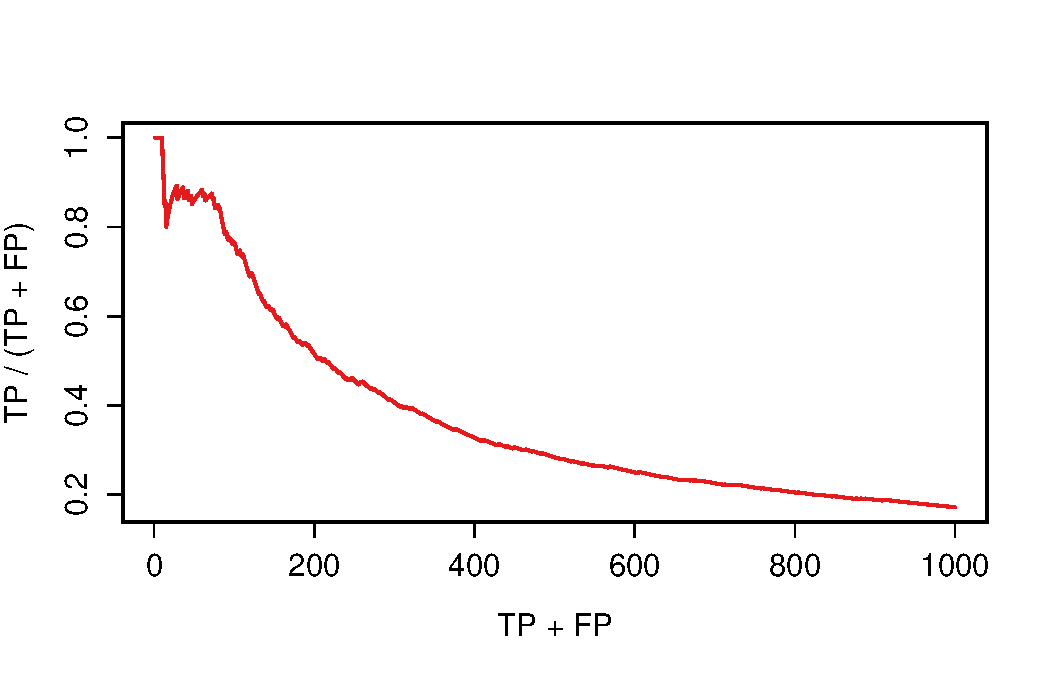
\includegraphics[width=\maxwidth]{figure/twocolumn-TP_plot-1} 

}

\caption[ ]{ }\label{fig:TP_plot}
\end{figure}
\end{Schunk}
	
	% 4
	\paragraph{4}
	The parameter $\theta$ sets, as previously hinted, the similarity percentage cutoff between sequences. In our case, as it is set to $\theta = 0.3$, only sequences with more than $1.0 - 0.3 = 0.7 = 70~\%$ similarity will be processed when calculating the weights. This makes it so that, according to the aforementioned equation, sequences which are very similar will add less to the corresponding weights, as the information is duplicated in several parts of the input data, which here are the homologues. By doing so, we smoothen our distribution of weights, and thus makes it more variable due to smaller variation. We can also note how changing the $\theta$ parameter somewhat removes the initial bump, signifying that the initial dip indeed is because of low-abundance pairs distorting the prediction.
	
	% question 5
	\paragraph{5}
	Pseudocounts are used for smoothing distributions in particular when some specific probabilistic outcomes are unlikely to occur in relation to the size of the data set. In the case of amino acids, this could be to add and increment to the number of times a residue has been observed. For each amino acid, a different increment would be attributed, based on a prior estimates of how likely they are to appear. This approach is done in order to avoid sharp peaks in the distribution of values in for example a position weight matrix, where small changes in the number of observations would have large effects the resulting value, in the case where pseudocounts are not used. In practice, pseudocounts can be set to calculate the posterior estimator of the mean as
	\begin{equation*}
		\theta^{PME}_i = \dfrac{n_i + \alpha_i}{|\mathbf n| + |\mathbf \alpha |}
	\end{equation*}
	where $n_i$ is the number of observations of component $i$, and $\alpha$ is the pseudocounts for that component~\cite{durbin1998biological}.
	
	% The pseudocounts roughly reflect the chances of seeing the amino acid in a context in which we have not previously seen it. A low pseudocount for an amino acid means that the amino acid is not often seen in a context in which some other amino acid has already been observed. If the pseudocount is lower than we would expect from the background probabilities, then the amino acid must be more highly conserved than other amino acids. Using this reasoning, we expect that G, P, W, and C are often highly conserved. Using symmetric reasoning for pseudocounts that are higher than expected from the background probabilities,   we also expect that M, Q, and S are less conserved than other amino acids.
	
	\paragraph{6}
	\Cref{fig:varying} shows the changes in predictability when changing the two parameters. As we can note, changing the pseudocount weight appears to saturate at around $0.6$. Having values under this makes the model underperform, where the lowest pseudocount weight leads to the worst performance. When instead keeping the pseudocount weights constant and instead changing $\theta$, we see that there is a balancing act between extracting the vital information and managing not to throw it out. As we can see from the figure, only very little of the material is needed to be discarded in order to get a good estimate in this case.
\begin{Schunk}
\begin{figure}[H]

{\centering 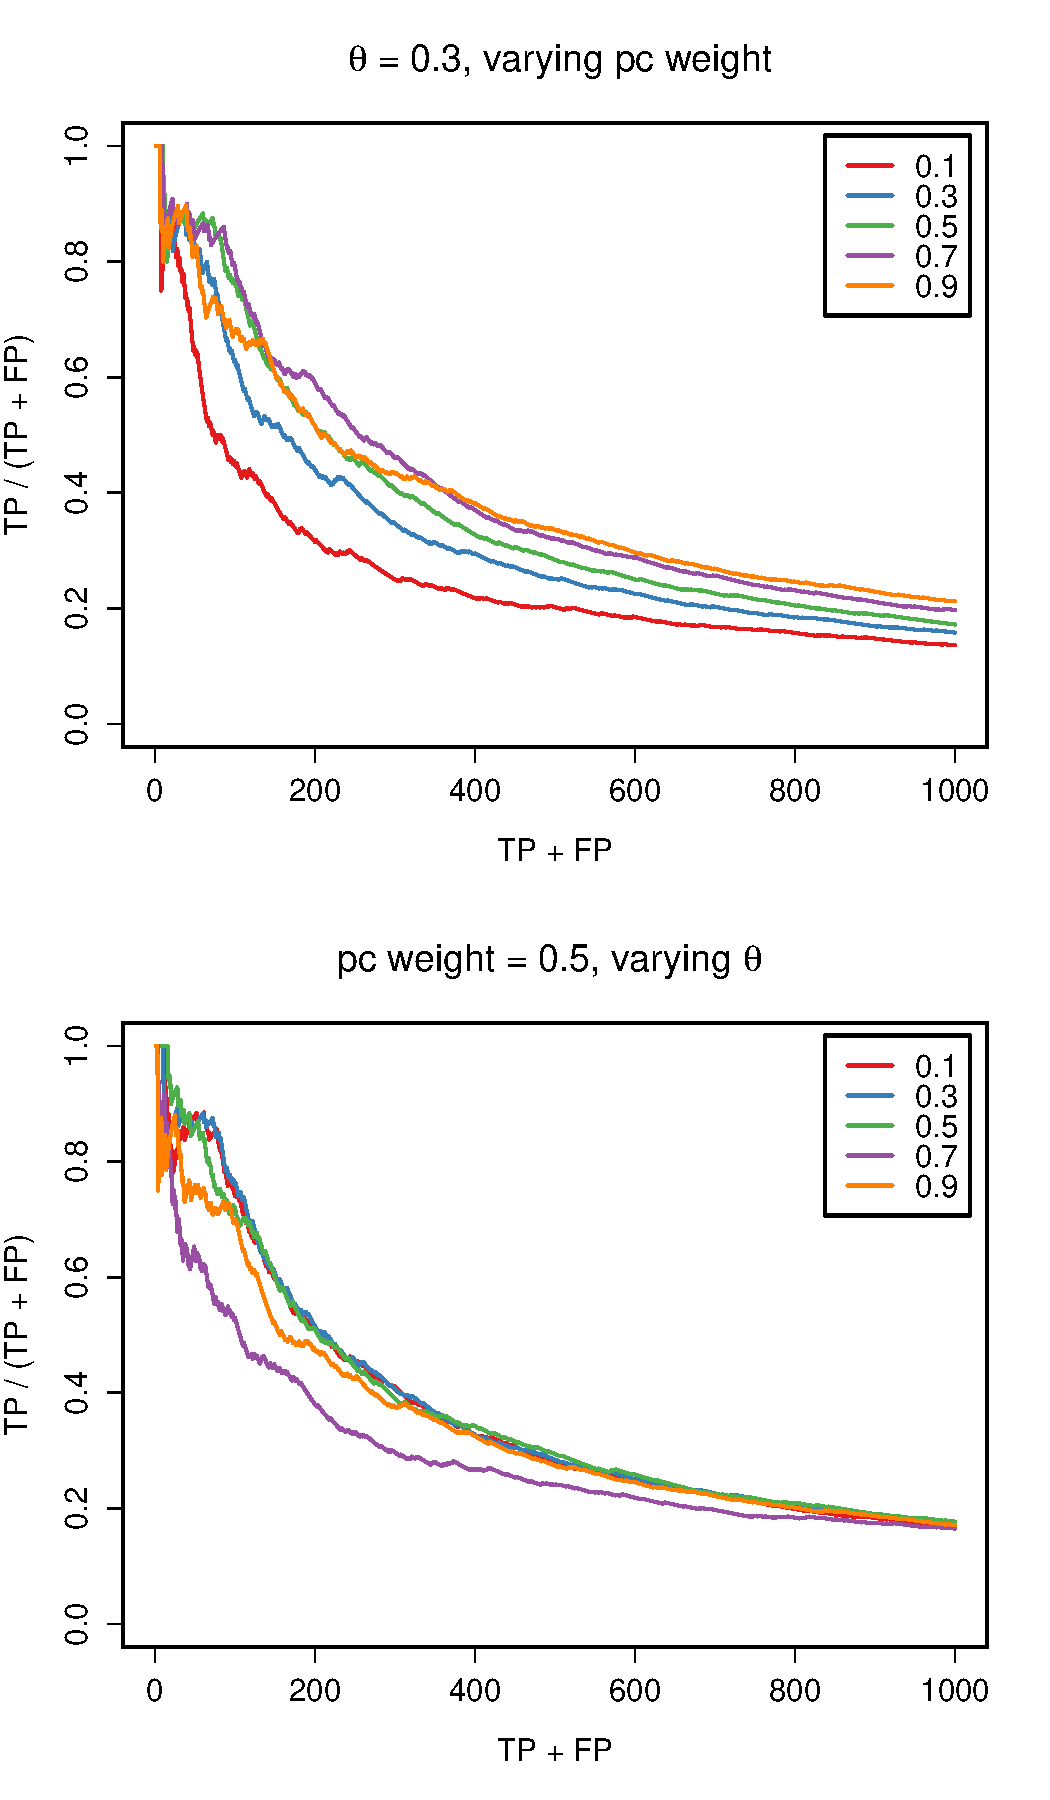
\includegraphics[width=\maxwidth]{figure/twocolumn-varying-1} 

}

\caption[ ]{ }\label{fig:varying}
\end{figure}
\end{Schunk}
	
	In \cref{fig:sensandso} we can observe the sensitivity and precision for pseudocount weights and $\theta$ both in the range $[0, 1]$. While the minimum is clearly identifiable, there is no homogeneous slope towards it. Nevertheless, we 
	
\begin{Schunk}
\begin{figure}[H]

{\centering 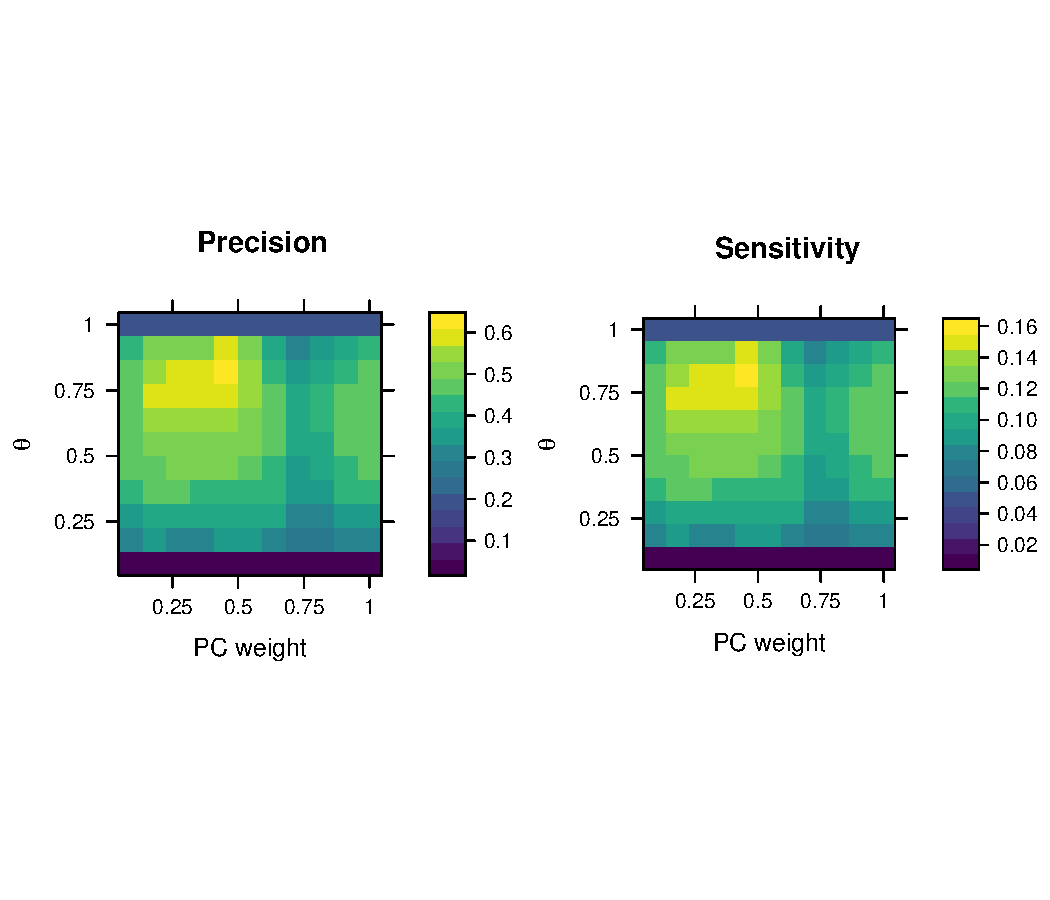
\includegraphics[width=\maxwidth]{figure/twocolumn-sensandso-1} 

}

\caption[ ]{ }\label{fig:sensandso}
\end{figure}
\end{Schunk}
	
	\paragraph{7}
	When comparing the three different proteins with each other using the default parameters we get the results shown in \cref{fig:otherprot}. Notably, LACI\_ECOLI performs the best, with the other bacterial species coming after. The human protein performs the worst in general. The origin of the Human protein is as it is simply because the highest ranked prediction is a false positive. 
\begin{Schunk}
\begin{figure}[H]

{\centering 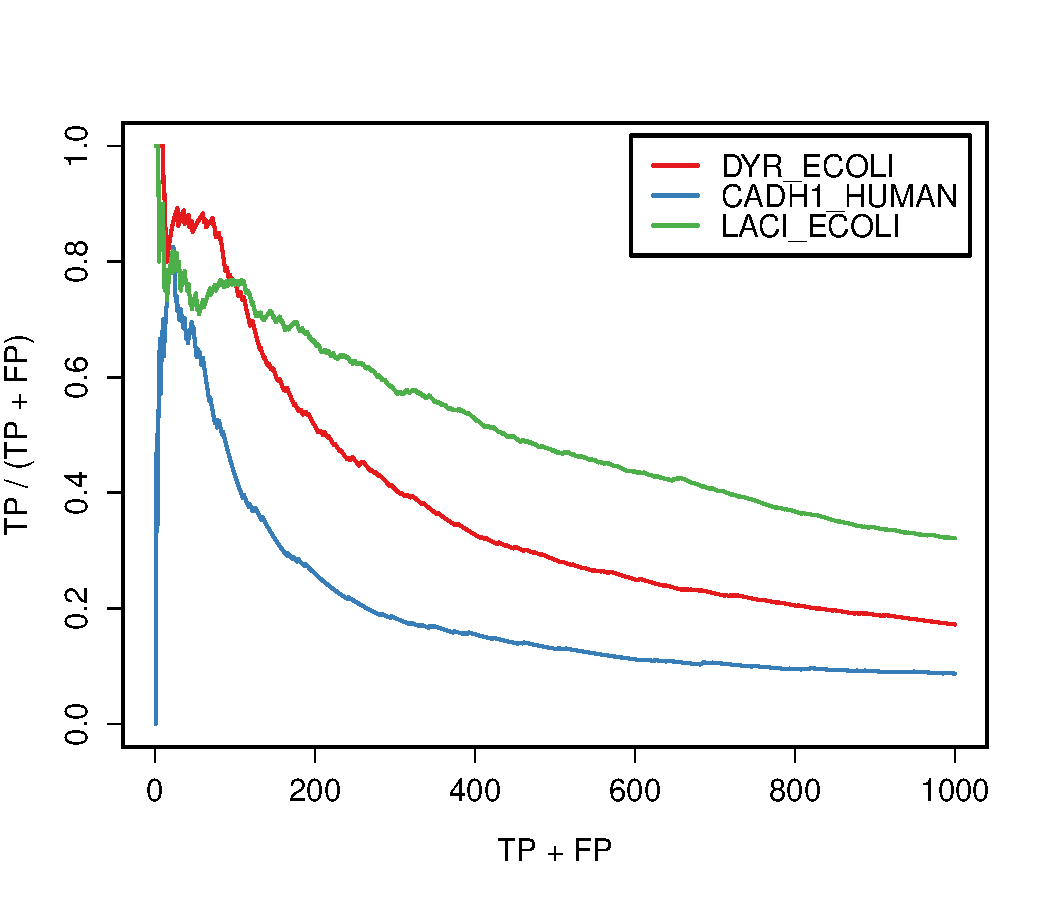
\includegraphics[width=\maxwidth]{figure/twocolumn-otherprot-1} 

}

\caption[ ]{ }\label{fig:otherprot}
\end{figure}
\end{Schunk}
	
	\paragraph{8}
	% Question	8:	How	do	you	expect	performance	to	vary	as	the	length	of	the	protein	
	% sequence	being	analysed increases?	What	do	you	find	from	the	true	positive	
	% plots	that	you	have	generated?	
	Given \cref{fig:otherprot}, we can tie this information to the sequence lengths. From our data, we have that our data for LACI\_ECOLI contains sequences of at most 360 residues, whereas CADH1\_HUMAN has a more modest length of 151, and DYR\_ECOLI of 159. Normally, we would expect sequences of longer lengths to match worse due to the increased risk of missmatches and tendency to include non-functional residues. When the sequences are longer, the low-abundance subsequences will also cause the distribution landscape to be rougher and hence not as robust in performance.
	
	However, in our figure, we see the opposite effect, where longer sequences generally have higher predictive quality, aside from a discrepancy for high-scoring pairs. This could be because of different degrees of variance between homologs in our species, due to for example insertions and deletions. Indeed, a visual check on this affirms that the biological variance between the three cases is significant, with in particular DYR\_ECOLI being generally very well conserved, whereas CADH1\_HUMAN suffers from more indels than the ECOLI counterparts. It is also the case that LACI\_ECOLI has the most sequences included in the data set, which might simply entail that the difference we see is due to a relative lack of data in the other cases.
	
	\paragraph{9}
	% Question	9:	Given	your	findings	in	question	7,	and	your	answers	to	questions 4	
	% and	5 above,	do	you	think	the	same	parameter	values	should	be	used	for	all	of	
	% these	proteins,	given	the	input	data	that	you	have	been	provided	with? If	you	
	% were	given	a	new	protein	to	analyse,	what	factors	would	affect	your	choice	of	
	% parameter	values	for	theta	and	pc_weight?	
	
	Using the same parameters is clearly not a satisfying solution due to the differences in biological variance (and subsequently the error in alignment). There are naturally also differences in the frequency of the amino acids, which directly should affect the distribution of pseudocounts and their relative importance. For a new protein, it would be beneficial to take into account the factors previously mentioned, such as sequence lengths, variance in this, and conservation and variance in the corresponding subsequences.
	
	% No. They should depend on how frequent the amino acids are, and how high variance there is between the homologs. 
	
	\paragraph{10}
	% Question	10: What	factors	other	than	the	available	input	data	might	cause	the	
	% accuracy	of	contact	prediction to	vary	between	different	proteins?	To	answer	
	% this	question,	you	should	refer	to	your	findings	in	this	assignment	so	far,	to	the	
	% papers	provided	on	moodle	with	this	assignment,	and	in	addition any	other	
	% material	you find	relevant.	
	
	The accuracy of the method depends inherently on the quality of the sequence alignment, and as a consequence then on the method used for aligning. Ideally, dynamic programming would render the mathematically optimal fit between the sequences, although the large number of sequences makes it computationally impossible for any substantial studies. This means that heuristic methods must be applied in order to speed up the alignment, and the design and choice of these are thus bound to affect the quality of the alignment. Taking into account as much available data as possible, for example about the insertion/deletion frequencies and the abundance of the various k-mers can then be used to improve upon this~\cite{thompson1994clustal}. 
	
	Similarly to this, still relating to the sequences, is the accuracy of the data itself, e.g.\ in the case of the 3D structure. Many proteins have structures which are difficult to capture precisely, which means that the sequence data and the corresponding fold sometimes are not very reliable, and depends on the method used to capture the conformation~\cite{pena77consensus,rakesh2016improving}.
	
	Aside of the sequences themselves, our approach does not take into account environmental factors, such as interacting ligands and ions which might aid or obstruct certain types of folds and change the overall folding trajectory. While highly correlated pairs might have importance in folding and making the protein reaching the native state, our method is unable to account for the fact that this does not happen in an isolated environment~\cite{marks2012protein}. 
	\bibliography{references}
\end{multicols*}
	\newpage
\appendix
	%%%%%%%%%%%%%%%%%%%%%%%%%%%%%%%% DYR  
	\begin{figure*}[t]
		\centering
		\phantom{p}
		\begin{subfigure}[b]{.49\textwidth}
			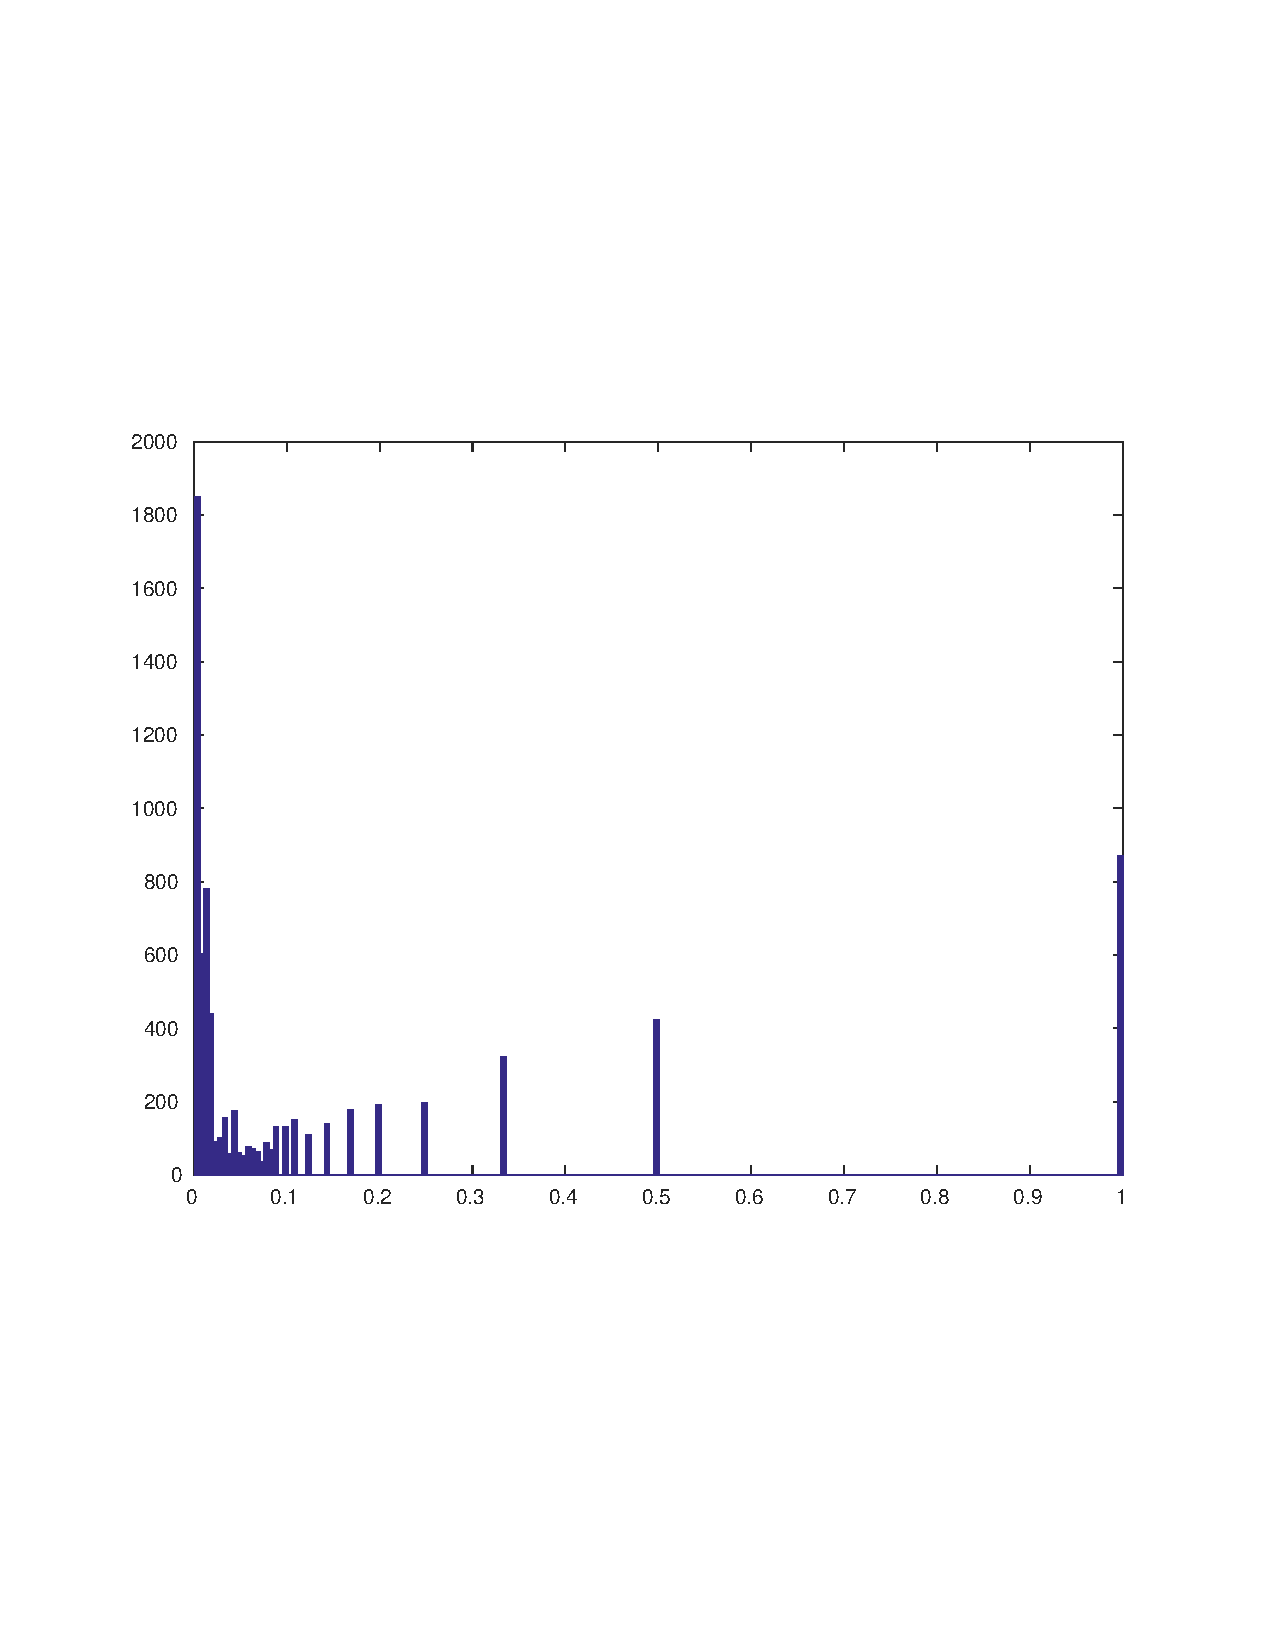
\includegraphics[width=\textwidth, trim = 2cm 6cm 2cm 6cm, clip]{{../figures/DYR_ECOLI_e3_n2_m40_theta_0.3_pc_weight_0.5_histogram_}.pdf}
			\caption{ }
			\label{fig:dyr_fig1}
		\end{subfigure}~
		\begin{subfigure}[b]{.5\textwidth}
			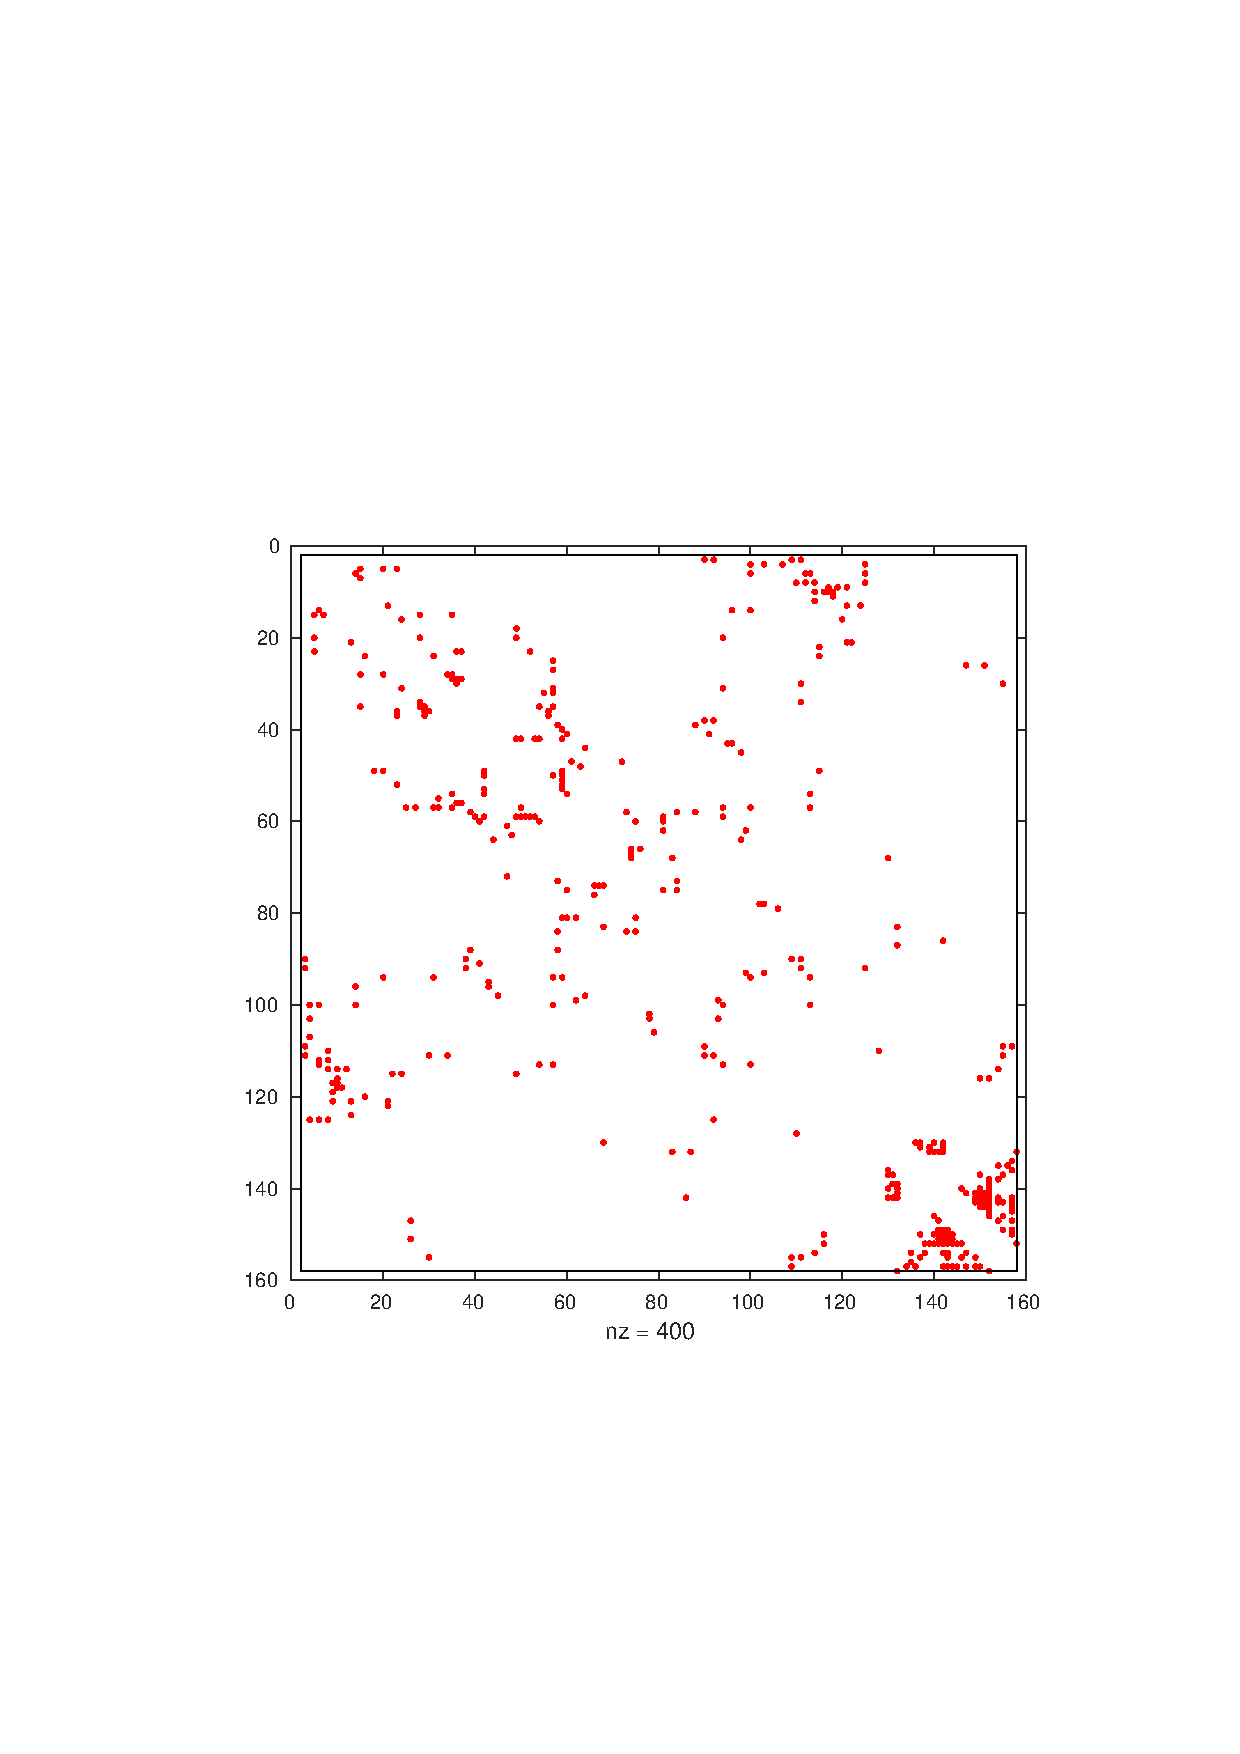
\includegraphics[width=\textwidth, trim=2cm 7cm 2cm 7cm, clip]{{../figures/DYR_ECOLI_e3_n2_m40_theta_0.3_pc_weight_0.5_Predicted_Constraints}.pdf}
			% 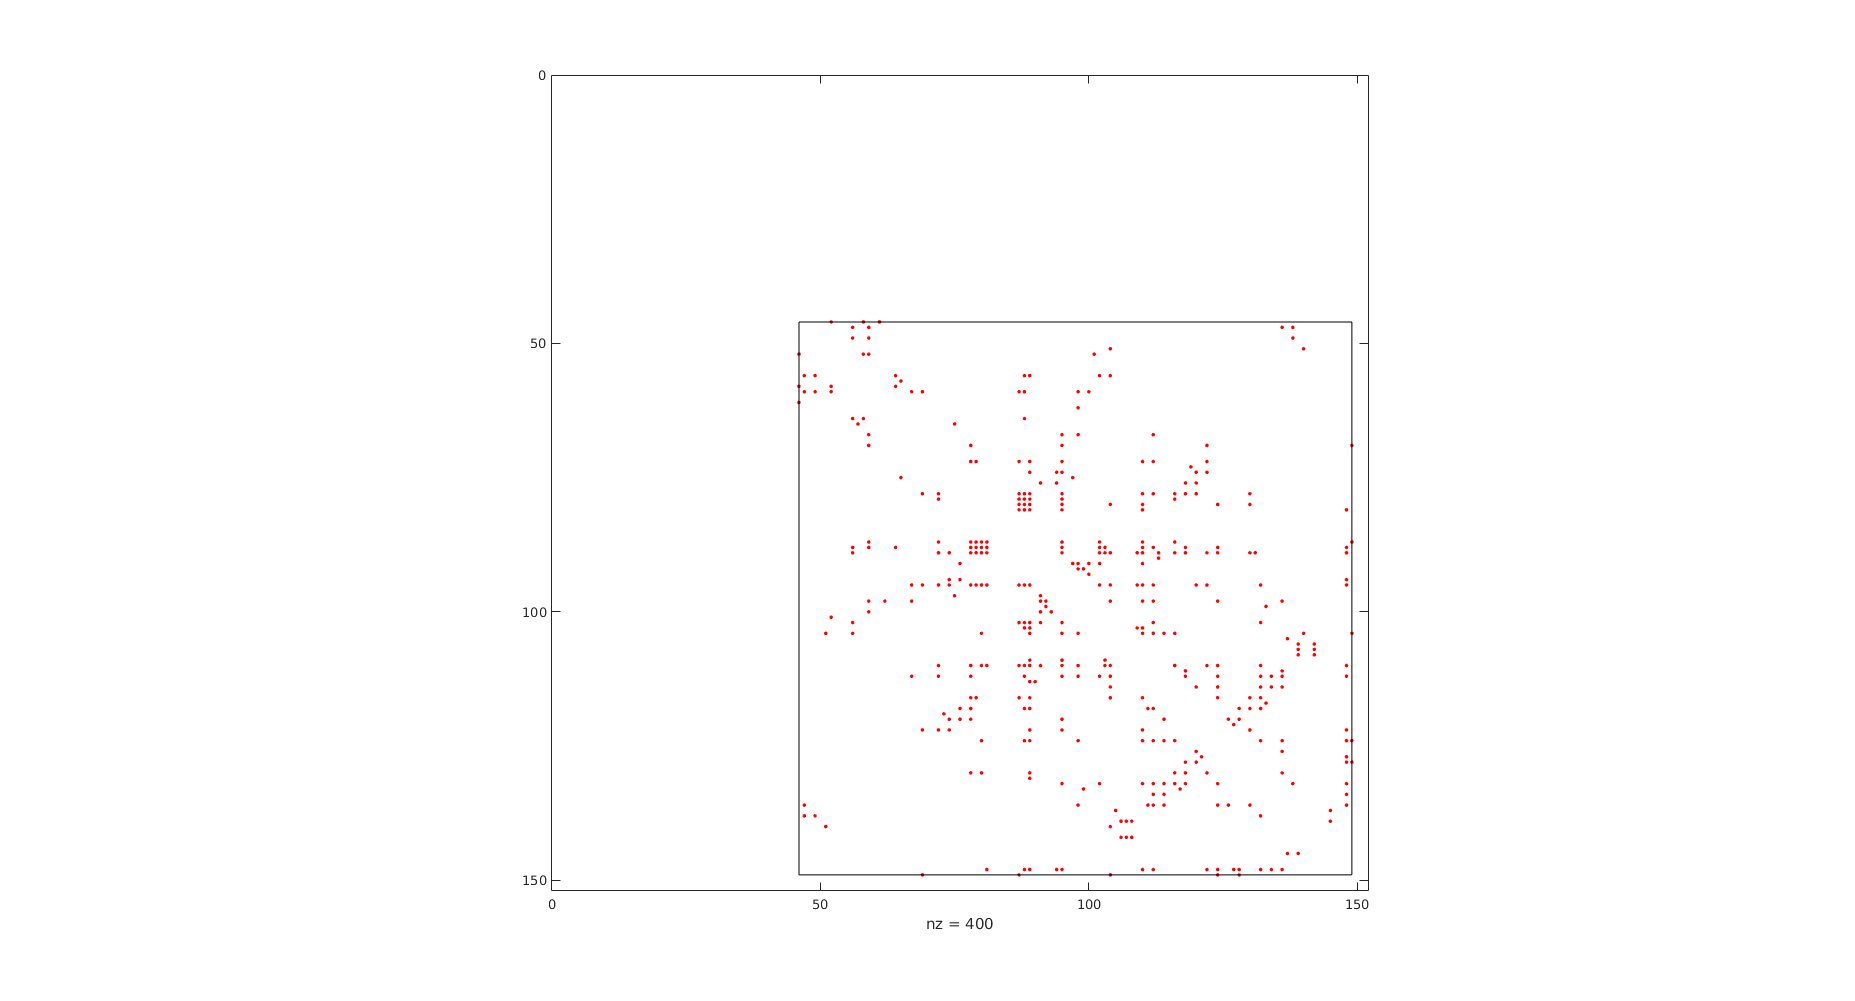
\includegraphics[width=\textwidth, trim= 10cm 0 10cm 0, clip]{../figures/fig2}
			\caption{ }
			\label{fig:dyr_fig2}
		\end{subfigure}\\
		\begin{subfigure}[b]{.49\textwidth}
			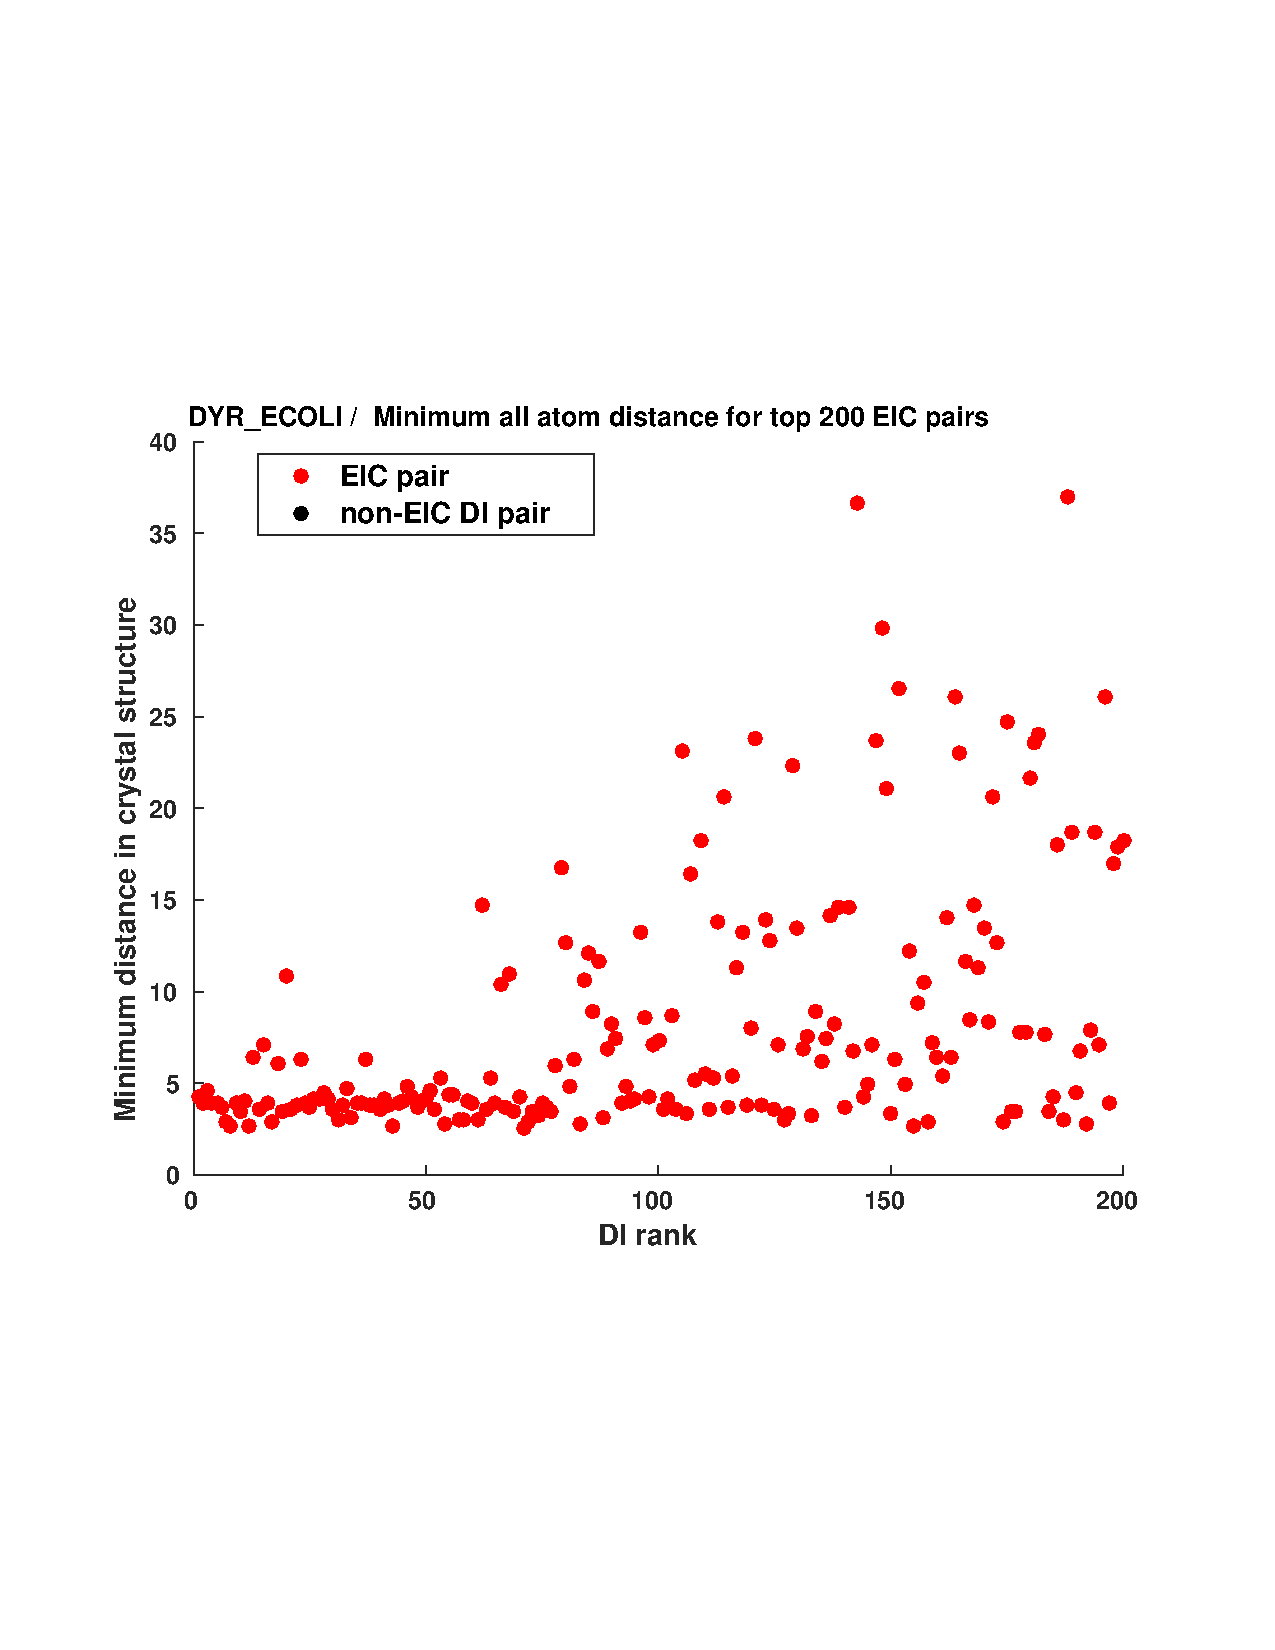
\includegraphics[width=\textwidth, trim= 2cm 7cm 2cm 0cm, clip]{{../figures/DYR_ECOLI_e3_n2_m40_theta_0.3_pc_weight_0.5_FPplot}.pdf}
			\caption{ }
			\label{fig:dyr_fig3}
		\end{subfigure}~
		\begin{subfigure}[b]{.5\textwidth}
			% 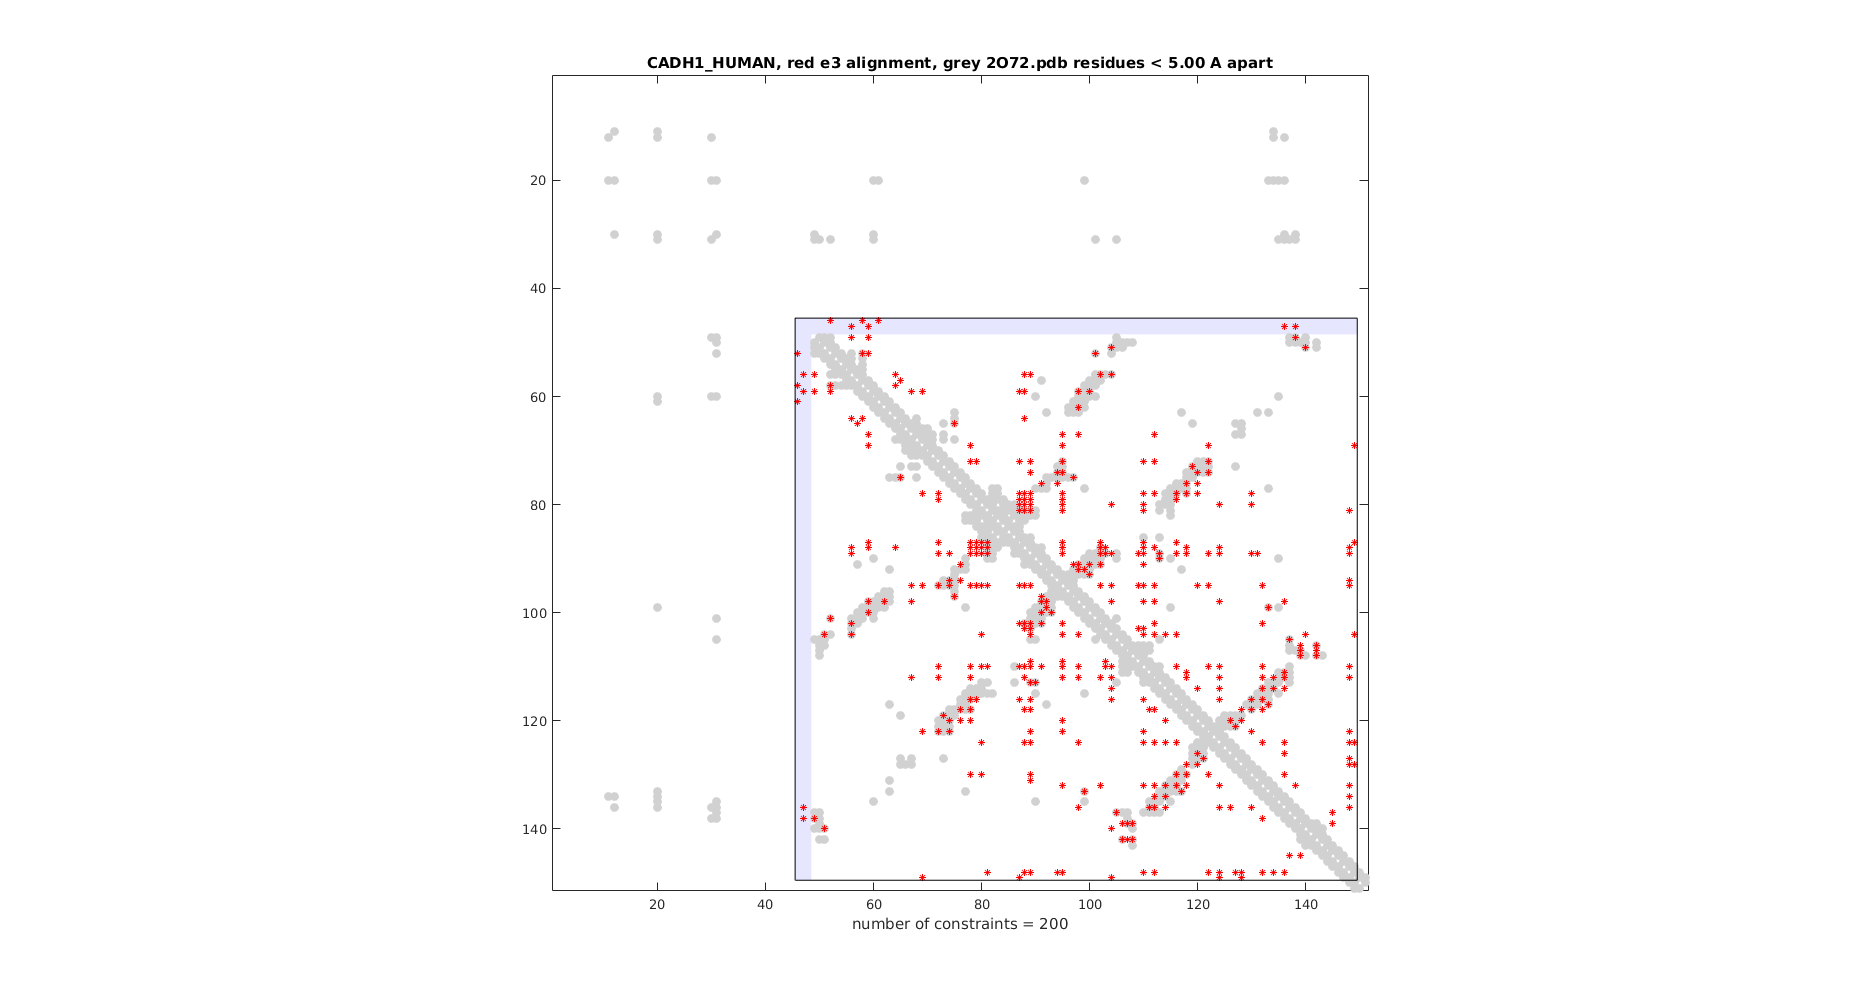
\includegraphics[width=\textwidth, trim= 10cm 0cm 10cm 0, clip]{../figures/fig4 }
			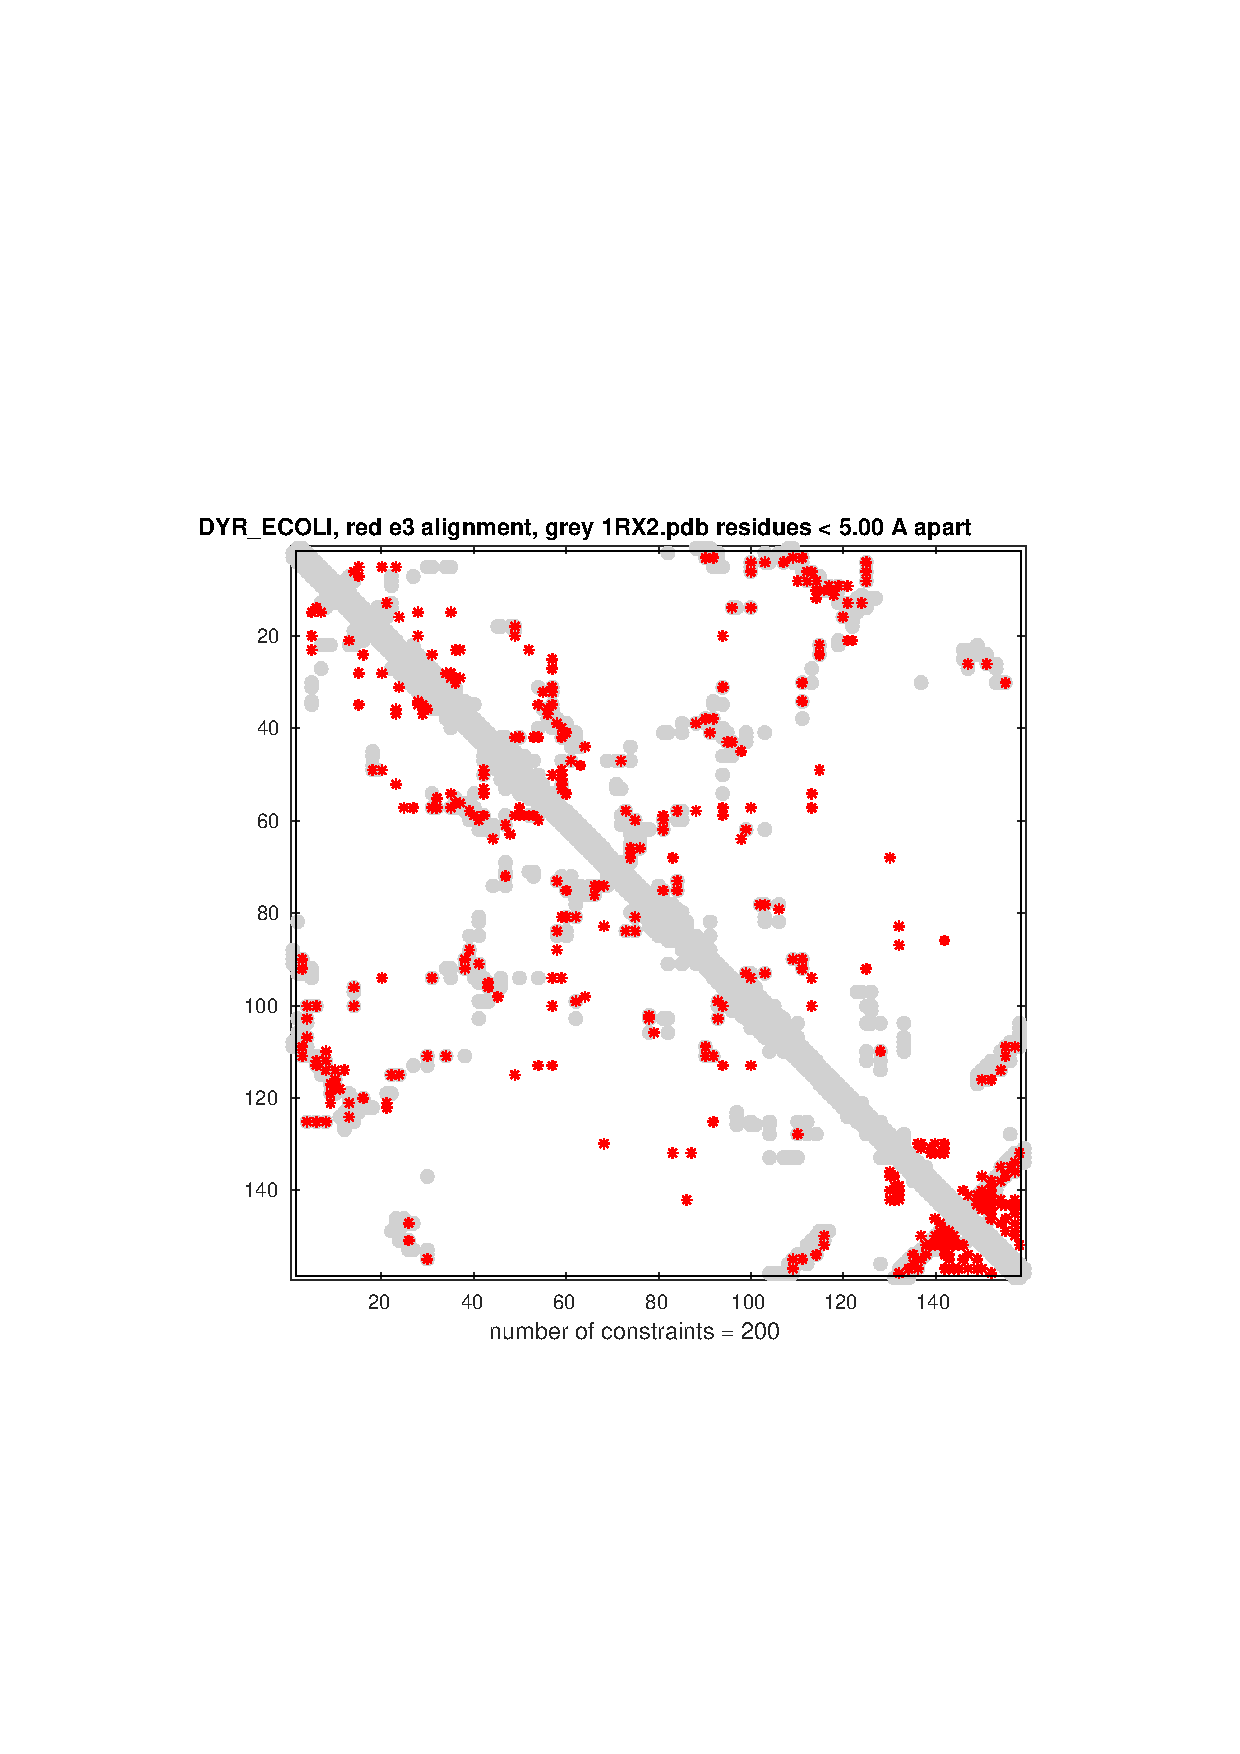
\includegraphics[width=\textwidth, trim=2cm 7cm 2cm 7cm, clip]{{../figures/DYR_ECOLI_e3_n2_m40_theta_0.3_pc_weight_0.5_Cmap_200}.pdf}
			\caption{ }
			\label{fig:dyr_fig4}
		\end{subfigure}%
		\caption{ }
		\label{fig:dyr_init_figures}
	\end{figure*}

\section{Code}
  \lstinputlisting{../code/exc_3.R}
  \lstinputlisting{../code/exc_6.R}
  \lstinputlisting{../code/tp_plot.R}
  \lstinputlisting{../code/varying.R}


\end{document}
